\label{sec:metrics}

Once defined the coding schemes behavior in terms of encoding
and decoding, we proceed to describe the metrics considered in our study.
The goodput is a measure for the effective processing speed since it
excludes protocol overhead but considers all delays related with
algorithmic procedures, field operations, hardware processing, multicore
coordination (where it applies), etc. Moreover, encoding and decoding
goodput permits to observe if coding is a system-block that limits the
end-to-end performance. If a system presents a low goodput, this will
affect the \ac{QoE} of delay-intolerant applications for the end user.
For example, mobile user applications are typically delay-intolerant.
Furthermore, Raspberry Pi processors are based in the \ac{ARM} architecture
which is the same as in mobile devices such as smartphones or tables.
Thus, the Raspberry Pi might be used as an experimental tool to get an
estimate of a mobile device processing capability which is easy-deployable
and at a much lower cost than a smartphone.

To complement our study, we review the energy consumption of the Raspberry
Pi since this platform is deployed at a large scale in scenarios where (i)
energy is constrained to the lifetime of the device battery and (ii) the
devices could be established in locations that are unavailable for
regular maintenance. Typical use cases of this type of scenarios are
sensor applications where devices are positioned for measurement retrieval
without any supervision for large periods fo time.

\subsection{Goodput}
We consider the goodput defined as the ratio of the useful delivered
information at the application layer and the total delivery time. We focus
on the goodput considering only the coding process, i.e. we assume that
the application data has been properly generated before encoding and
also correctly post-processed after decoding. In this way, we define
the goodput for either an encoder or a decoder as follows:
%
\begin{align} \label{eq:goodput}
Goodput = \frac{gB}{T_{proc}} ~ [\mathrm{Bytes/s}]
\end{align}
%
In \eqref{eq:goodput}, $B$ and $g$ are the packet and generation size
as defined previously and both represented the data to be processed. For
goodput measurements, we are concerned in quantifying the processing time
for either encoding or decoding $g$ \ac{l.i.} packets. Thus, $T_{proc}$ is
the processing time required for this processing. In the next subsections, we
define two time bechmarks available in [\textbf{Chres repos here}].
The purpose of the benchmarks is to quantify the processing time for
any of the coding scheme considered in Section \ref{sec:schemes}.

\subsubsection{Encoding Benchmark}
Fig. \ref{fig:enc_goodput_benchmark} refers to the benchmark setup
made for measuring the encoding processing time. The time benchmark
is divided in two parts. In the first part, called a \textit{pre-run},
we quantify the amount of \textit{transmitted} coded packets from an
encoder (named 1 in Fig. \ref{fig:enc_goodput_benchmark}) required for
decoding in a single encoder-decoder link with no packet erasures
for a defined configuration of coding scheme, coding parameters and
amount of feedback. In the case of \ac{TSNC}, we also record the
points where a feedback was received from the decoder. The purpose of
the pre-run is to predict how an encoder should behave with a given
seed within its random number generator. This part of the benchmark is
not regarded as a measurement.

In the second part which is the actual \textit{simulation}, a reseted
encoder (2 in Fig. \ref{fig:enc_goodput_benchmark}) is given the same
seed as in the pre-run and then we measure the time from which the
process start until we reach the amount of transmitted packets in the
pre-run. Then, this measurement is stored as the encoder $T_{proc}$
for this generic configuration.

\begin{figure}[ht!]
\centering
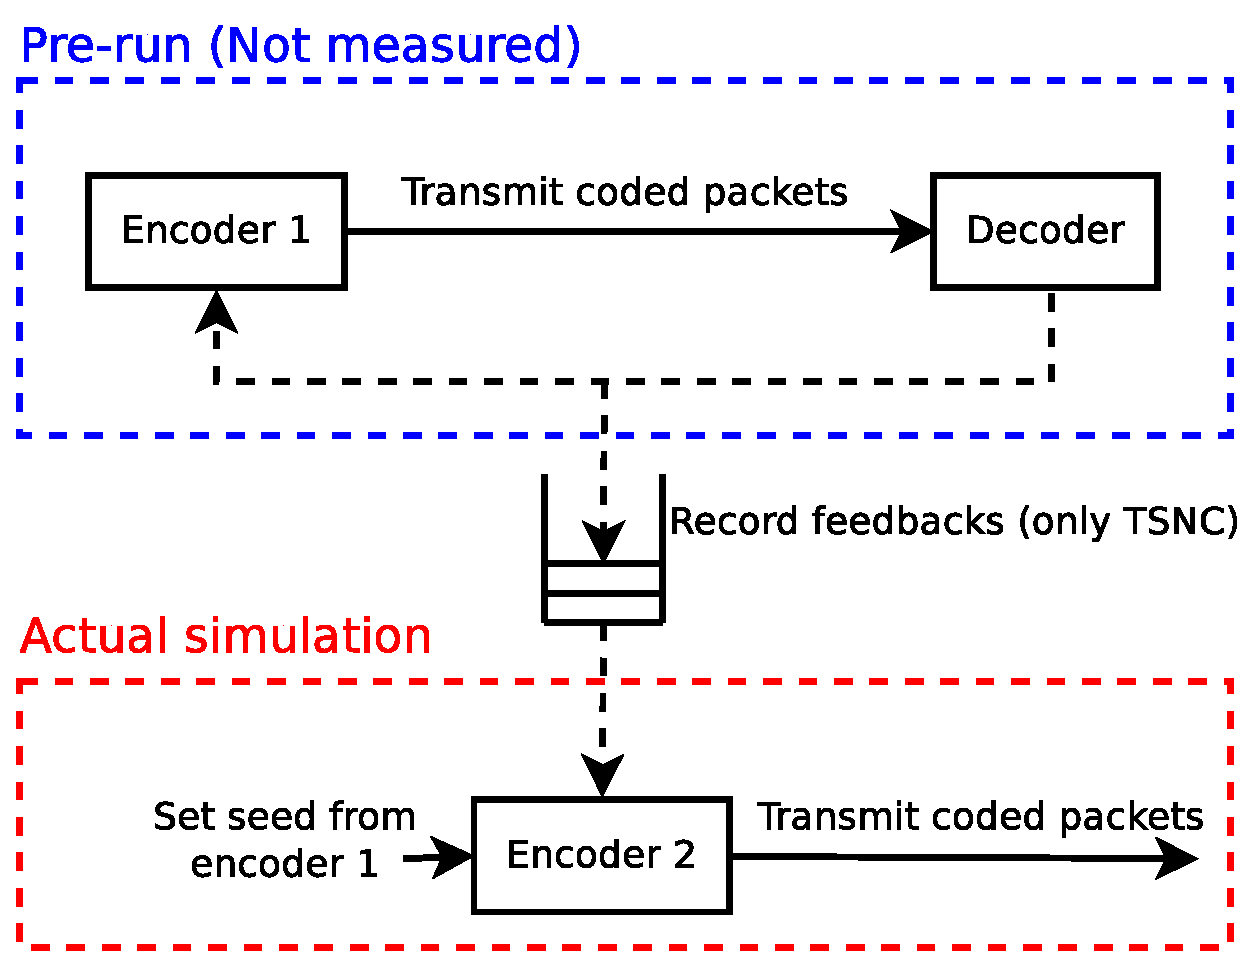
\includegraphics[width=0.6\textwidth]{images/measure_encoder.eps}
\caption{Encoding goodput benchmark}
\label{fig:enc_goodput_benchmark}
\end{figure}

\subsubsection{Decoding Benchmark}
Fig. \ref{fig:dec_goodput_benchmark} shows the benchmark setup
for measuring the decoding processing time. The time benchmark
is divided in two parts as its encoding counterpart, e.g. a pre-run
and the actual simulation. However, some differences occur.

In the pre-run, we still quantify the amount of transmitted coded
packets from encoder 1. Notice that we include the feedback case because
it is necesary for the \ac{TSNC} scheme. However, now we store
the \textit{transmitted packets} instead. The reason being
that we want to feed the decoder with the same packets in the same
order. Later, in the actual simulation, an encoder (2 in Fig.
\ref{fig:dec_goodput_benchmark}) is given the same packets in the same
order from the pre-run and then we measure the time from which the
process start until the decoder finishes to retrieve the original
packets. Finally, this measurement is saved as the decoder $T_{proc}$
for this general configuration.

\begin{figure}[ht!]
\centering
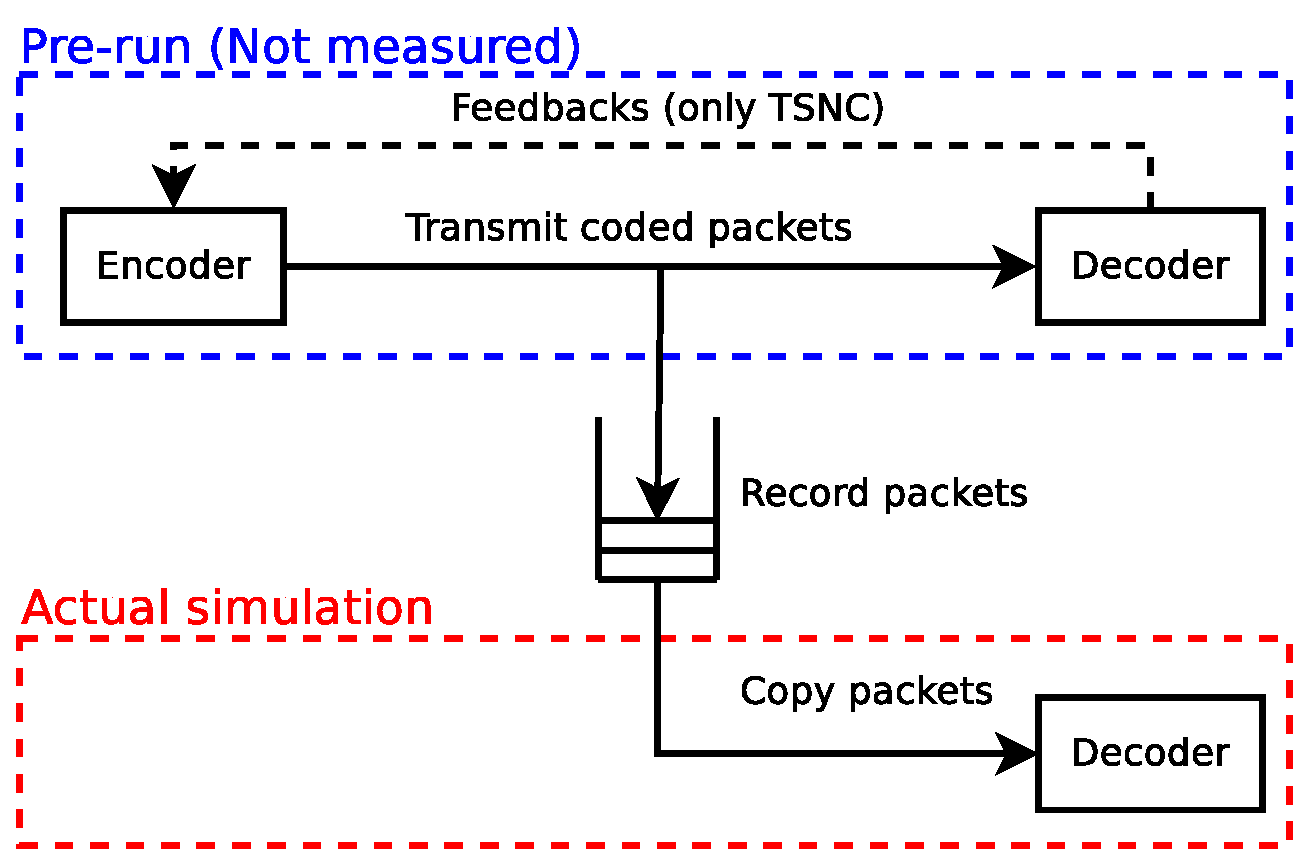
\includegraphics[width=0.6\textwidth]{images/measure_decoder.eps}
\caption{Decoding goodput benchmark}
\label{fig:dec_goodput_benchmark}
\end{figure}

\subsection{Energy Consumption}
In large-scale networks where several Raspberry Pis might be deployed,
both overall and per-bit energy consumption of the devices during the
encoding and decoding process are relevant parameters that impact in the
network performance for a given coding scheme. To compute the

\subsubsection{Average}
\subsubsection{Per-Bit}